\subsection*{Сумма ряда -- синус}
\addcontentsline{toc}{subsection}{Сумма ряда -- синус}

\textbf{Задание:}\\
Используя диаграмму действий, реализовать алгоритм вычисления сумм ряда синуса.\\

\textbf{Решение:}\\
Для вычисления экспоненты воспользуемся суммом ряда Тейлора:
\[\sin x \approx \sum_{k = 0}^{N} (-1)^k \dfrac{x^{2k+1}}{(2k+1)!} \]

В соответствии с данной формулой была построена рекуррентная формула для вычисления данной суммы. (Рисунок \ref{fig:sin1})
\begin{figure}[h]
	\centering 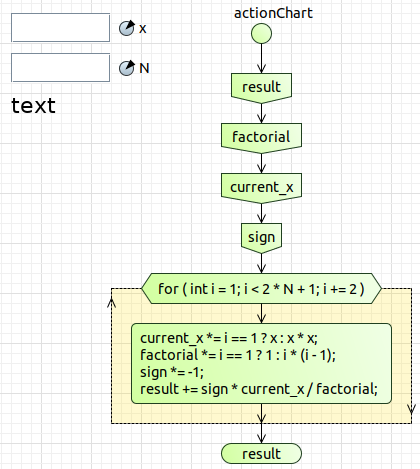
\includegraphics[scale=0.5]{sin1}
	\caption{Диаграмма действий для суммы ряда синуса}
	\label{fig:sin1}
\end{figure}

На вход данному алгоритму поступает количество итераций и степень $x$. (Рисунок \ref{fig:sin2})
\begin{figure}[h]
	\centering 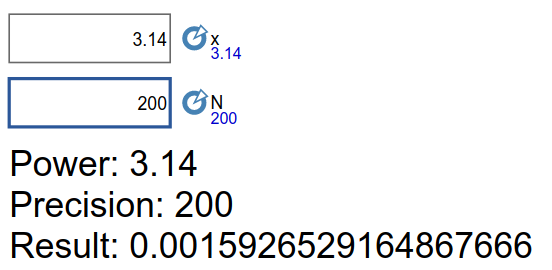
\includegraphics[scale=0.21]{sin2}
	\caption{Результаты вычисления ряда синуса}
	\label{fig:sin2}
\end{figure}

\newpage

Результаты расчёта совпали с результатами Wolfram Mathematica.\\

Таким образом, на примере создания функции для нахождения суммы ряда синуса был освоен процесс работы с диаграммами действий.